\documentclass{article}
\usepackage[left=2cm,right=2cm,top=2cm]{geometry}

\usepackage{amsmath}
\DeclareMathOperator*{\argmax}{arg\,max}
\DeclareMathOperator*{\argmin}{arg\,min}

\usepackage{amsthm,amsmath,amssymb}
\usepackage[numbers]{natbib}
\usepackage{hyperref}
\usepackage{graphicx}
\usepackage{caption}
\usepackage{subcaption}
\newcommand{\bx}{{\mathbf x}}
\newcommand{\ba}{{\mathbf a}}
\newcommand{\bv}{{\mathbf v}}
\newcommand{\bu}{{\mathbf u}}


\newtheorem{theorem}{Theorem}[section]
\newtheorem{proposition}[theorem]{Proposition}
\newtheorem{lemma}[theorem]{Lemma}
\newtheorem{corollary}[theorem]{Corollary}
\newtheorem{remark}{Remark}[section]
\newtheorem{example}[theorem]{Example}


\begin{document}

\title{Management Sciences Topics: Convex Optimization\\ Homework 3}
\date{}
\maketitle

\begin{enumerate}
\item Problem 1

We may change the step size to
$$
\eta_k = \frac{2}{\mu(k+2)}
$$
as when $\mu > 0$ in SSG. Now we show that

First, by three term lemma,
$$
\langle x^{k+1}-x^k, g_x^k\rangle + \frac{1}{2\eta_k}\lVert x^{k+1}-x^k\rVert_2^2 \le \langle x-x^k, g_x^k\rangle + \frac{1}{2\eta_k}\lVert x-x^k\rVert_2^2 - \frac{1}{2\eta_k}\lVert x-x^{k+1}\rVert_2^2.
$$
By strong convexity of $f$ w.r.t. $x$,
$$
f(x^k, y) - f(x^*, y) \le \langle g_x^k, x^k - x^*\rangle - \frac{\mu}{2}\lVert x^k - x^*\rVert_2^2.
$$
Then by mean inequality,
$$
\begin{aligned}
f(x^k, y) - f(x^*, y) &\le \langle x^*-x^k, g_x^k\rangle +\frac{1}{2\eta_k}\lVert x^*-x^k\rVert_2^2-\frac{1}{2\eta_k}\lVert x^*-x^{k+1}\rVert_2^2-\frac{1}{2\eta_k}\lVert x^{k+1}-x^k\rVert_2^2 -\frac{\mu}{2}\lVert x^k-x^*\rVert_2^2 \\
&\le \frac{1}{2}\eta_k \lVert g_x^k\rVert_2^2 + (\frac{1}{2\eta_k}-\frac{\mu}{2})\lVert x^k-x^*\rVert_2^2-\frac{1}{2\eta_k}\lVert x^*-x^{k+1}\rVert_2^2 \\
&\le \frac{1}{2}\eta_k M^2 + (\frac{1}{2\eta_k}-\frac{\mu}{2})\lVert x^k-x^*\rVert_2^2-\frac{1}{2\eta_k}\lVert x^*-x^{k+1}\rVert_2^2 \\
&= \frac{1}{\mu(k+2)}M^2 +\frac{\mu k}{4}\lVert x^k-x^*\rVert_2^2 - \frac{\mu(k+2)}{4}\lVert x^*-x^{k+1}\rVert_2^2.
\end{aligned}
$$
Then
$$
\sum_{k=0}^{K-1}(k+1)(f(x^k, y) - f(x^*, y)) \le \sum_{k=0}^{K-1} \frac{k+1}{\mu(k+2)}M^2 + \sum_{k=0}^{K-1} \frac{\mu k(k+1)}{4}\lVert x^k-x^*\rVert_2^2 - \sum_{k=0}^{K-1} \frac{\mu(k+1)(k+2)}{4}\lVert x^*-x^{k+1}\rVert_2^2,
$$
and
$$
\frac{k(k+1)}{2}(f(\bar{x}, y)-f(x^*, y)) \le \frac{KM^2}{\mu},
$$
so
$$
f(\bar{x}, y)-f(x^*, y) \le \frac{2M^2}{(k+1)\mu}.
$$
Similarly, we have
$$
f(x, \bar{y})-f(x, y^*) \le \frac{2M^2}{(k+1)\mu}.
$$
Lets $y = \bar{y}$ in the first equation and $x = x^* $ in the second equation, by adding these two equations, we get
$$
f(\bar{x}, \bar{y}) - f(x^*, y^*) \le \frac{4M}{(K+1)\mu}.
$$
Then the algorithm has a convergence rate of $O(\frac{1}{k})$.


\item Problem 2.
By Nesterov smoothing,
$$
h_\mu(x) = \max_{\lVert y_g\rVert_2 \le 1} \tilde{h}(y) = \max_{\lVert y_g\rVert_2 \le 1} \lambda y^\top Cx - \frac{1}{2}\mu\lVert y\rVert_2^2,
$$
where the index $g$ is for all groups, and $C$ is the group matrix.

Take partial derivative w.r.t. $y$,
$$
\frac{\partial}{\partial y}\tilde{h}(y) = \lambda Cx - \mu y.
$$
Then the maximizer is
$$
y_g^* = S_2(\frac{\lambda (Cx)_g}{\mu}),
$$ 
where $S_2 $ is the projection operator onto the unit $L_2 $ ball. Then
$$
h_\mu(x) = \lambda y^{*\top} Cx - \frac{1}{2}\mu \lVert y^*\rVert_2^2,
$$
and from Theorem 1 of https://arxiv.org/ftp/arxiv/papers/1202/1202.3708.pdf,
$$
\nabla h_\mu(x) = C^\top y^*,
$$
and the Lipschitz constant for $\nabla h_\mu $ is $L = \frac{1}{\mu}\lVert C\rVert_2^2 $.

Now we consider the problem as follows:
$$
f = g+h, 
$$
where 
$$
g = \frac{1}{n}\sum_{i=1}^{n}\log(1+\exp(-b_ia_i^\top x))+\lambda y^{*\top} C x - \frac{1}{2}\lVert y^*\rVert_2^2,
$$
and 
$$
h = 1_{\mathcal{X}}(x).
$$
Then the proximal of $\eta h$ is just the projection operator w.r.t. $\mathcal{X}$.

The code for this problem is \texttt{accelerated\_proximal\_gradient.m} and \\
\texttt{overlapped\_group\_regularized\_logistic\_regression\_smooth.m}. The objective value of average iterate is shown in Figure \ref{problem 2}.

\begin{figure}[h]
\centering
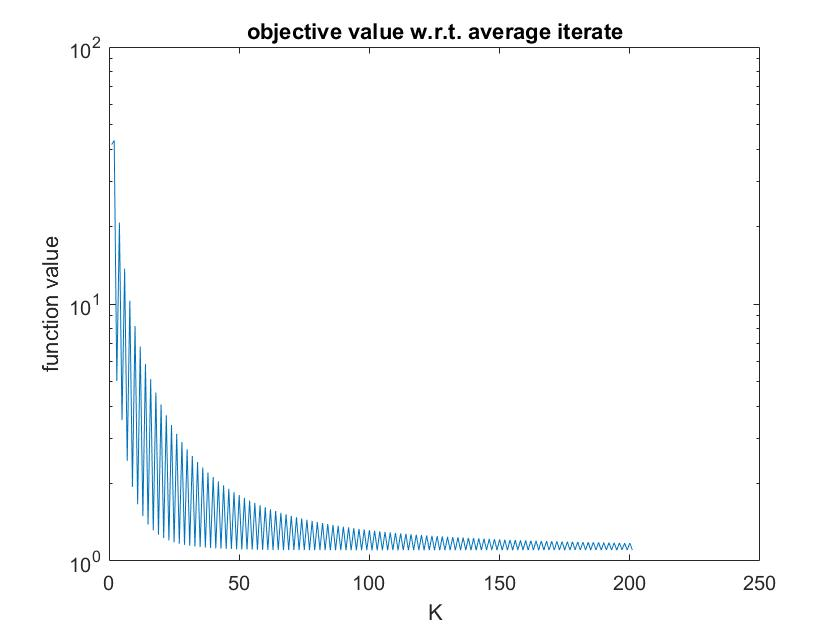
\includegraphics[scale=0.3]{problem2.jpg}
\caption{Objective value for problem 2.}
\label{problem 2}
\end{figure}


% Then 
% $$
% \text{Prox}_{\eta h_\mu}(x) = \argmin_{y} p(y) = \argmin_{y} \frac{1}{2}\lVert y-x\rVert_2^2 + \eta h_\mu(y),
% $$
% and the partial derivative is
% $$
% \frac{\partial}{\partial y}p = y-x + \eta\frac{\partial}{\partial y}h_\mu.
% $$
% We know from Theorem 1 of https://arxiv.org/ftp/arxiv/papers/1202/1202.3708.pdf that
% $$
% \frac{\partial}{\partial y}h_\mu = C^\top y^* = C^\top S_2(\frac{\lambda y}{\mu})
% $$
% where $C$ is the group matrix. Then since $h_\mu $ is smooth, the proximal is
% $$
% \text{Prox}_{\eta h_\mu}(x) = 
% $$

% Then the proximal $y = \text{Prox}_{\eta h_\mu}(x) $ must satisfies
% $$
% y - x + \eta C^\top S_2(\frac{\lambda y}{\mu}) = 0.
% $$



\item Problem 3.

The problem can be written as
$$
\min_{x}\max_y \frac{1}{n}\sum_{i=1}^{n}\log(1+\exp(-b_ia_i^\top x))+\lambda y^\top C x,
$$
where $C$ is the group matrix. Then pick
$$
g_x \in \partial_x f = \frac{1}{n}\sum_{i=1}^{n}\frac{-b_ia_i^\top\exp(-b_ia_i^\top x)}{1+\exp(-b_ia_i^\top x)} + \lambda C^\top y,
$$
and
$$
g_y \in -\partial_y (-f) = \lambda C x.
$$

The code for this problem is \texttt{primal\_dual\_subgradient.m} and \\ \texttt{overlapped\_group\_regularized\_logistic\_regression\_primal\_dual.m}. The objective value of average iterate is shown in Figure \ref{problem 3}.

\begin{figure}[h]
\centering
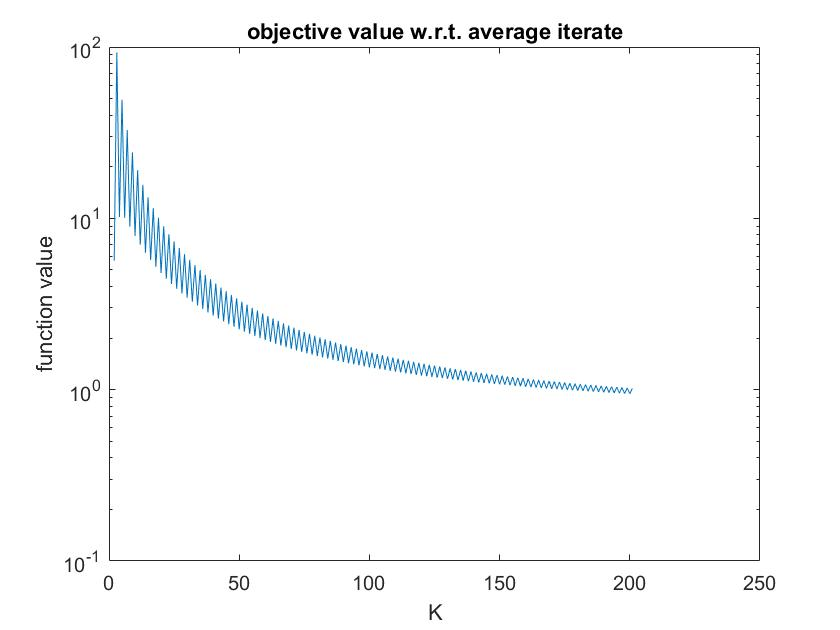
\includegraphics[scale=0.3]{problem3.jpg}
\caption{Objective value for problem 3.}
\label{problem 3}
\end{figure}


\end{enumerate}

\end{document}

